
\paragraph{Hexagonal Architecture}

Dentro de las arquitecturas de capas se va a realizar un diseño de puertos y adaptadores;
más conocido como arquitectura hexagonal.
El diagrama básico más utilizado en la teoría para representarlo se muestra en la ~\cref{fig:hexagonalDiagram}.
Este diagrama tiene un enfoque didáctico ya que el hexágono es una simple licencia estética.
En el caso de existir más puertos de salida o entrada que los representados, el hexágono pierde el sentido.
%Cuando se enfrenta por primera vez este diagrama se tiende a intentar descifrar el sentido oculto detrás de la elección de la forma poligonal, no existe.

\begin{figure}[H]
    \centering
    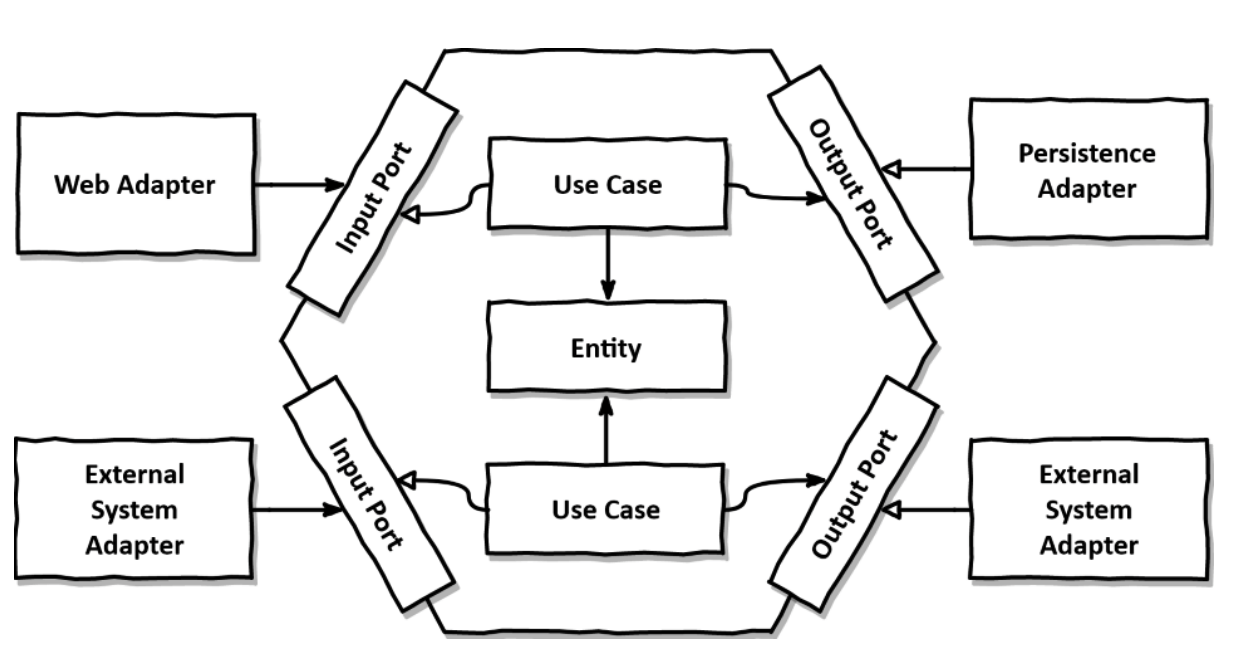
\includegraphics[height=0.22\textheight]{./part/Ejecucion/Seguimiento/CreateTaskUseCase/img/HexagonalDiagram}
    \caption{Ejemplo básico de un Diagrama de arquitectura hexagonal\cite{TomHombergs2019GYHD}}\label{fig:hexagonalDiagram}
\end{figure}

En este diagrama, el Dominio está representado por una única entidad, o \textit{Entity}, que se encuentra aislada de todo y no depende de ningún elemento.
La Aplicación está representada por los casos de uso, o \textit{Use Case}, y utiliza el Dominio dependiendo de él.
La Aplicación se aísla del exterior, la Infraestructura, obligando a utilizar sus interfaces a los elementos que acceden a ella.
Las interfaces son los elementos que bordean el hexágono nombrados como \textit{Input/Output Port}.
Utilizando estas interfaces, nombradas puertos, se encuentran los adaptadores o \textit{Adapters}.
Los Adaptadores de entrada, a la izquierda, utilizan directamente las interfaces, mientras que los de salida los implementan.
Representado por fechas con cabeza negra o blanca respectivamente.

En el diagrama~\cref{fig:layers} se aprecia este concepto simplificado.
La arquitectura hexagonal no es más que una arquitectura de capas que decide dividir el concepto de Infraestructura en dos tipos: la que hace uso de la Aplicación y la que la Aplicación utiliza.
El objetivo es expresar que la dependencia de las capas, expresada por las flechas, sea siempre de fuera hacia adentro.
Se preserva del cambio el interior y exponer al cambio el exterior.
Separar lo propenso al cambio de lo que no.
Separar el lenguaje propio del Dominio, \textit{Domain}, de los detalles de implementación, que tienen su propio lenguaje.

\begin{figure}[H]
    \centering
    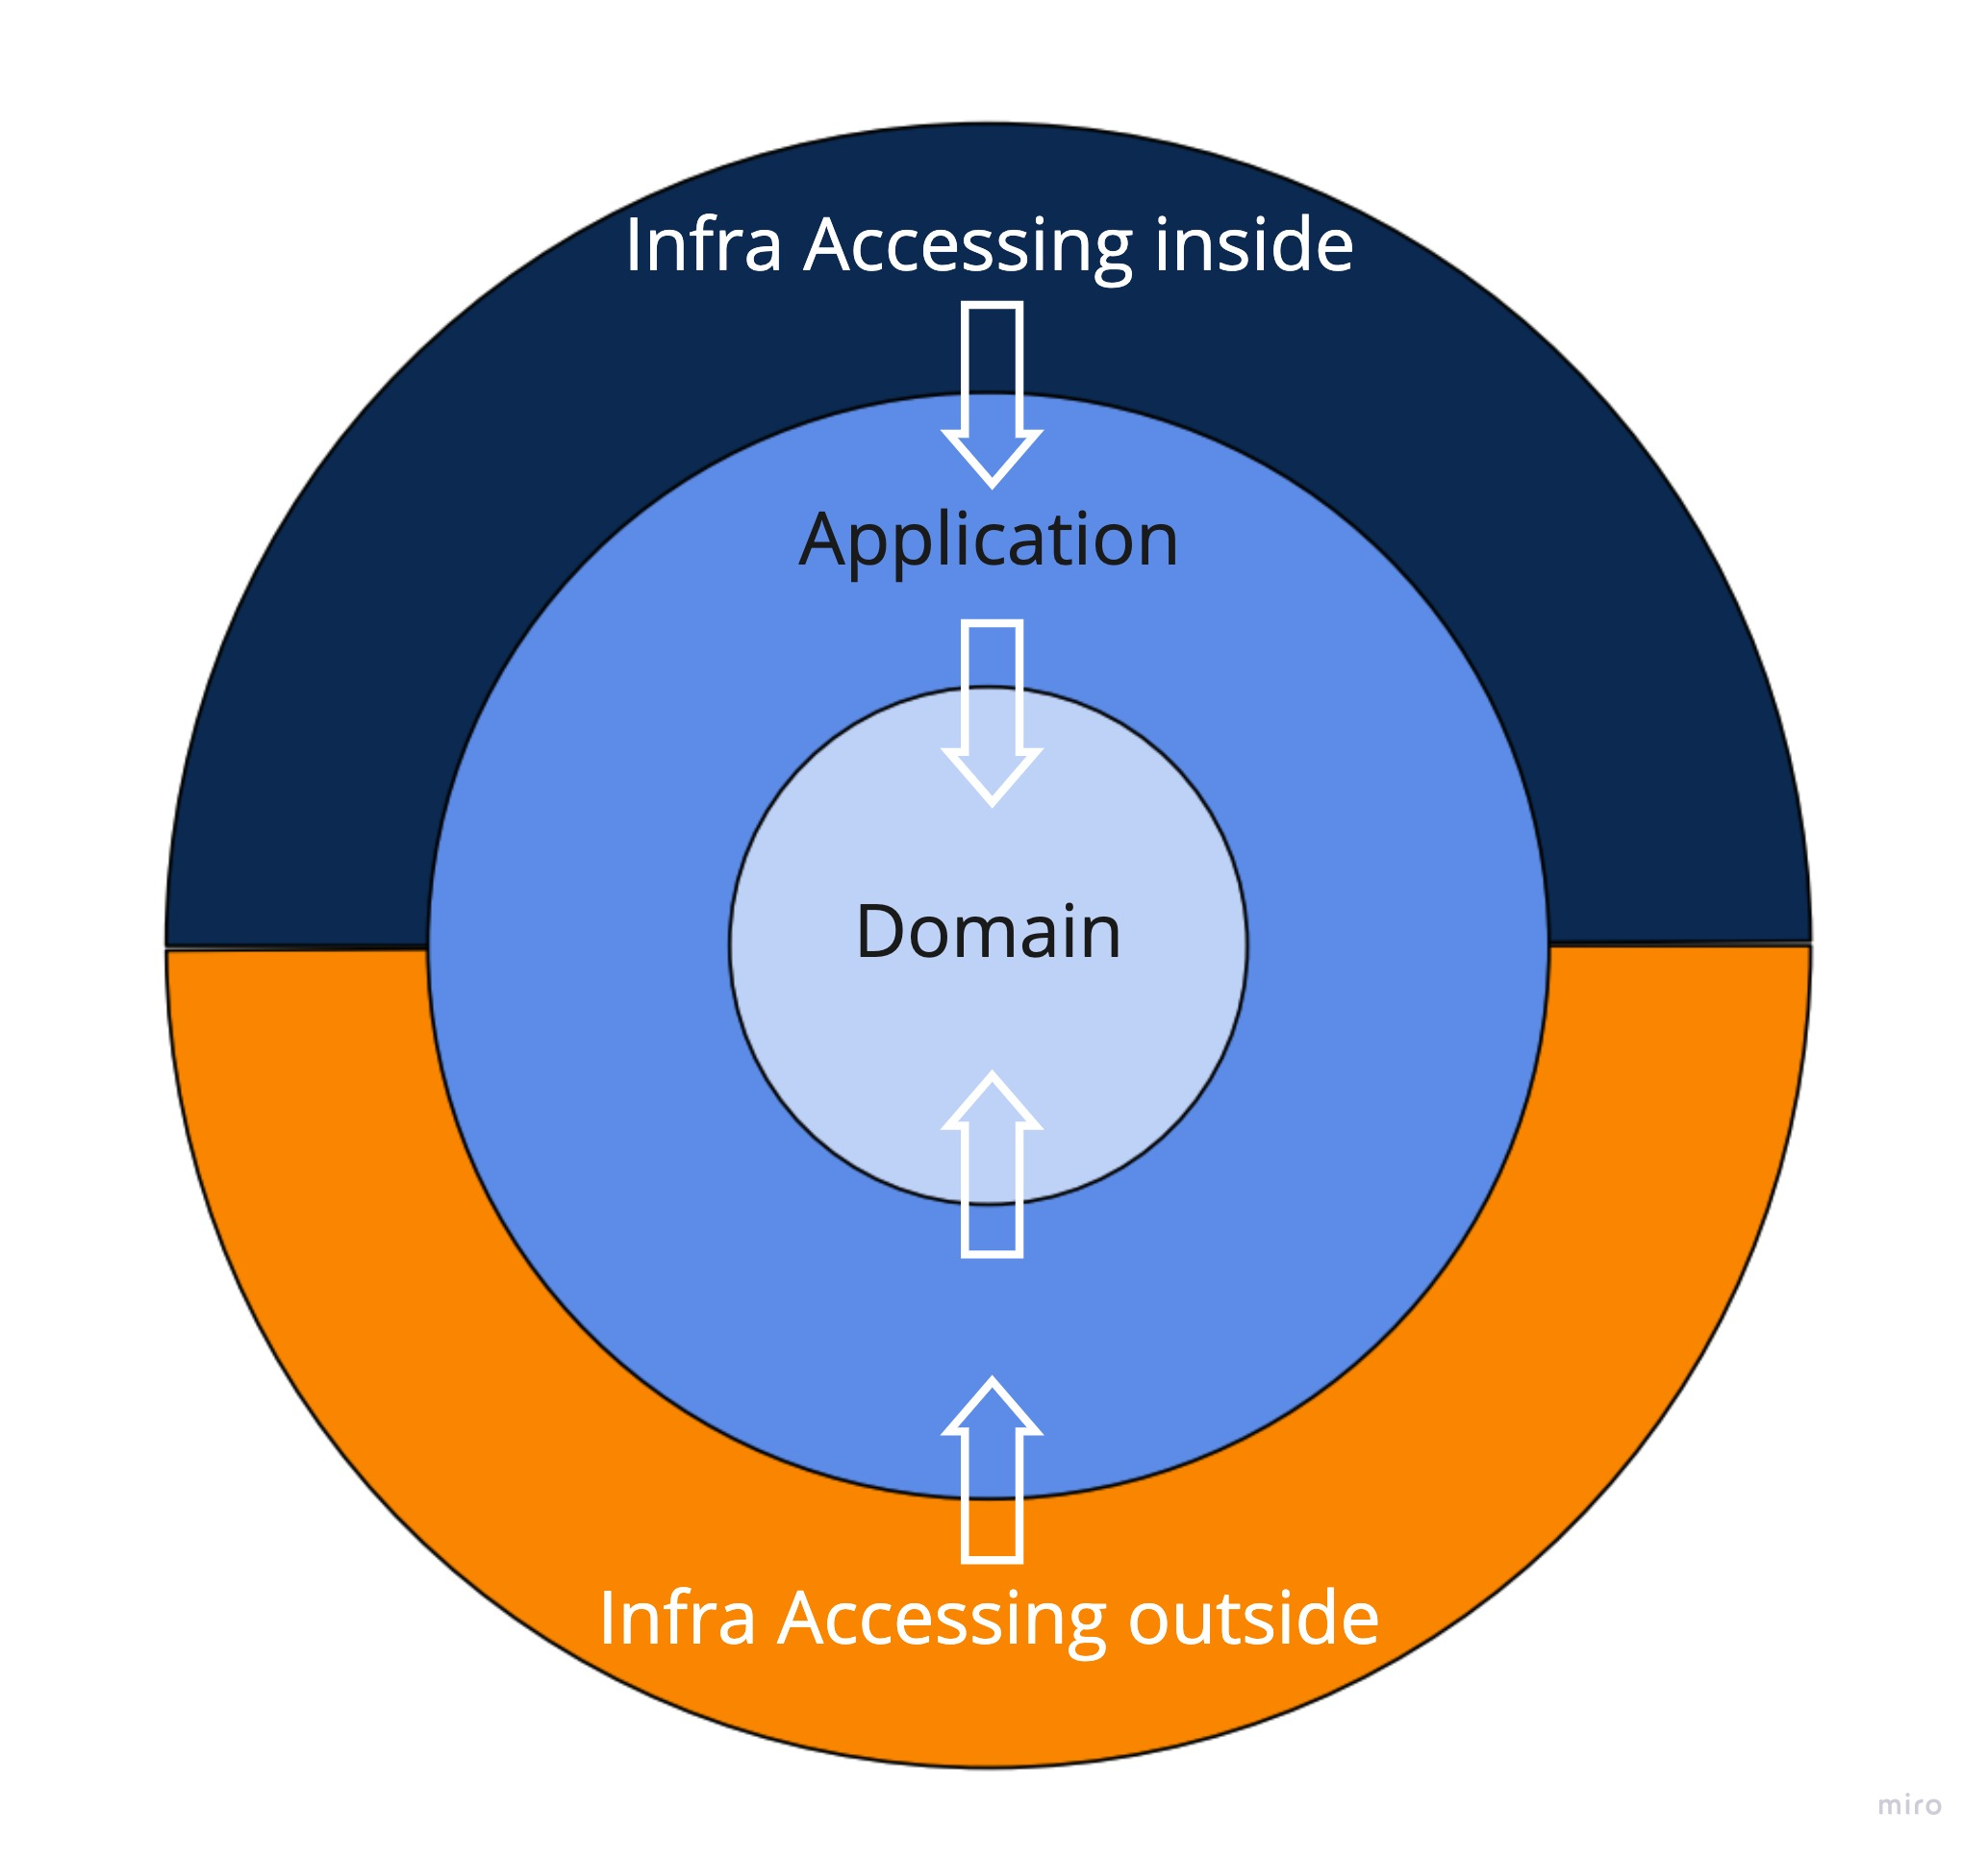
\includegraphics[height=0.22\textheight]{./part/Proyecto_ejecutivo/memoria_descriptiva/infoPreviaAntecedentes/img/PFM - Layer}
    \caption{Ejemplo básico de un Diagrama de arquitectura de capas}\label{fig:layers}
\end{figure}

\paragraph{Domain Driven Design}

\gls{DDD} (Domain-Driven Design o Diseño Dirigido por el Dominio) es una metodología de diseño enfocada a desarrollar un lenguaje común para todos los partícipes en un problema y su solución por ejemplo: clientes, vendedores, técnicos y financieros en un programa de gestión de venta de productos.
Para desarrollar ese lenguaje se divide el problema en contextos delimitados.

Por ejemplo en una empresa que comercialice actuadores automáticos: los actuadores para el equipo comercial significarán números de referencia y precios;
Para el departamento financiero significarán facturas y devoluciones;
Para los técnicos serán características físicas que los definen.
Si Los comerciales les llaman productos, los financieros les llaman concepto y los técnicos dispositivos, se encontrarán un problema de comunicación.
Realizar un software para la gestión de la empresa sin intentar resolver este problema de comunicación añade otra capa que además queda por escrita en el código.

%afiliado en un club deportivo significa facturas, números de identificación fiscal para los financieros y para la gente de operaciones significa reserva de pistas y cancelaciones.
%Para los de ventas significan descuentos, promociones, los demás actores tendrán otro significado para el mismo concepto.
%Todos utilizan la misma palabra para definir conceptos que difieren, pero cuando hablan de afiliados deben entenderse.
%Si en un departamento lo llaman clientes y en otro afiliados surgen problemas de comunicación.

Tener un lenguaje común donde todos puedan expresarse y hablar de la misma solución es el reto de este proceso.
Es lo que se define como \gls{UL} (Ubiquitous Language o lenguaje ubicuo) Intentar expresar en un mismo contexto todos esos significados termina en lo que se conoce como \textit{Big Ball of Mud} o Gran bola de barro.
Los componentes y las relaciones de este UL se pueden apreciar en la figura~\cref{fig:DomainDrivenDesignReference}.

Se describen los elementos que surgen del componente \textit{Model Driven Design}.
Que son los elementos dentro de ese lenguaje que afectan al diseño del software a su nivel más elemental:

\begin{itemize}
    \item \textit{Entity}: Elemento que contiene atributos definido por un identificador
    \item \textit{Value Object}: Elemento que tiene atributos pero no identificador
    \item Domain Event: Elemento que define una suceso inducido por la interacción entre los componentes del Dominio.
    \item Aggregate: Cluster de elementos tratado como una unidad.
    Las referencias o acciones externas sobre sus elementos siempre se hacen a través de un único elemento de este cluster conocido como \textit{Agreggate Root}.
    Tiene reglas definidas de consistencia dentro de su delimitación.
    \item Repository: Es un mecanismo de interacción para encapsular el acceso a tecnologías, como el almacenamiento en base de datos, para interactuar con ellas.
    La implementación no concierne al Dominio.
    \item Service: Es una funcionalidad de interacción entre elementos de Dominio.
    Encapsula lógica compleja que garantiza un comportamiento consistente.
\end{itemize}

Este paradigma de diseño compone el elemento central en el paradigma de la arquitectura de capas o \gls{LayerArchitecture}.
Se aíslan esos contextos que definen el Dominio de implementaciones concretas;
ya sea para acceder al Dominio o a las que accede el Dominio.
Por ejemplo, aislarlo de que se ejecute un servicio mediante una consola de comandos o desde una llamada http y que se guarde en una base de datos la información o se guarde en un archivo.

\begin{figure}[H]
    \centering
    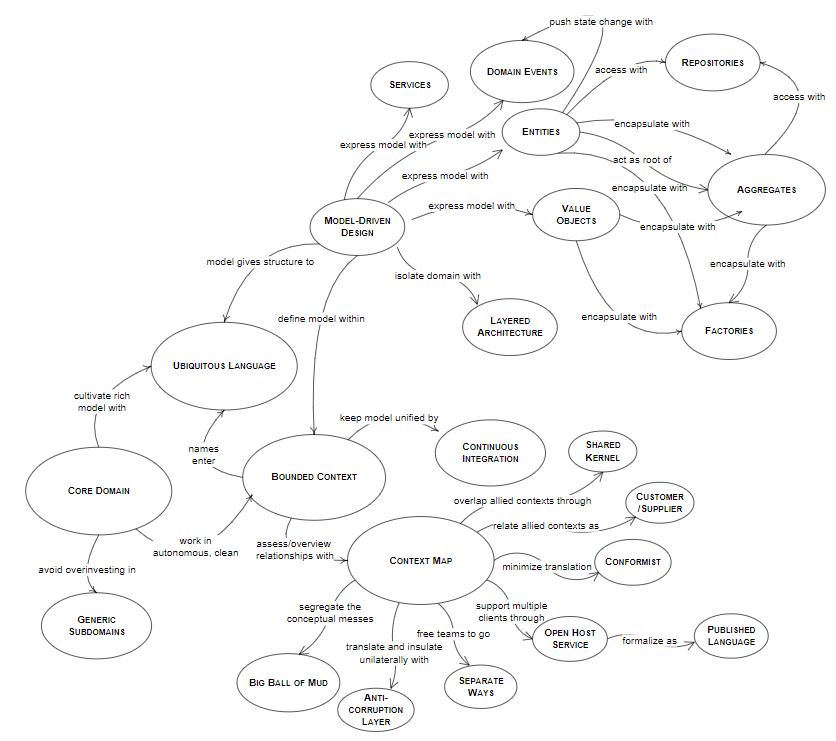
\includegraphics[height=0.6\textheight]{./part/Proyecto_ejecutivo/memoria_descriptiva/infoPreviaAntecedentes/img/DomainDrivenDesignReference}
    \caption{Diagrama conceptual de los elementos que componen DDD\cite{EricEvans2003DDTC}}\label{fig:DomainDrivenDesignReference}
\end{figure}

\paragraph{CQRS}

Junto con el concepto de arquitectura hexagonal y el \textit{DDD} se aplica el paradigma de diseño conocido como \gls{CQRS} (Command Query Responsibility Segregation).
Es una técnica de diseño de arquitectura de software que separa la lógica de escritura (comandos) de la lógica de lectura (consultas) en sistemas de información.
La idea es que las operaciones de escritura (comandos) y las operaciones de lectura (consultas) se manejen por separado, ya que tienen necesidades y características distintas.
Mientras que las operaciones de escritura son responsables de modificar el estado de la aplicación, las operaciones de lectura son responsables de devolver información sobre ese estado sin modificarlo.
Al separar estas dos responsabilidades, se pueden optimizar las operaciones de lectura para que sean más rápidas y escalables.
Además, se puede diseñar una arquitectura de software más flexible, permitiendo una mayor adaptabilidad y evolución del sistema a medida que cambian los requisitos de la aplicación.

El resumen hasta ahora es que el diseño sigue una arquitectura hexagonal, con un enfoque \textit{DDD} en el Dominio y un enfoque CQRS en los casos de uso.
Es decir se diseñará un Dominio rico y con un UL y se accederá a su funcionalidad a través de casos de uso que sigan el criterio de ser comandos y consultas.

\paragraph{\textit{Mapping} o Mapeo}

Otro paradigma de diseño para garantizar la separación efectiva de las capas en su uso de los elementos básicos con los que interactúan es el mapeo o el \textit{Mapping}.
Si un elemento de Infraestructura utiliza directamente una \textit{Entity} de Dominio estaría saltando la capa de Aplicación en su diagrama de dependencia.
Bien es cierto que se mantendría la dependencia de fuera hacia adentro, pero se ha de tomar una decisión de hasta qué punto se quiere desacoplar una capa de otra.
A esta decisión de diseño se le conoce como Estrategia de \textit{Mapping} entre capas.
Estrictamente cada capa requiere sus objetos de trabajo para estar desacoplada de las demás, pero como en todo aspecto de diseño está sometido a discusión acerca de seguir la teoría al pié de la letra y el pragmatismo de no verse envuelto en redundancias y sobredimensionar las soluciones.

Hay tantas estrategias como atajos dentro de este paradigma se desee asumir.
Habrá de enfrentarse a la decisión de diseño entre la teoría y a los atajos que se pueden tomar.
Evaluar los beneficios e inconvenientes y tomar una decisión con la que se ha de ser consecuente, y más importante en desarrollo, consistente.
Esto quiere decir que una vez tomada una decisión debe ser una decisión en equipo que todos sigan.
Es más eficiente un diseño imperfecto que sea consistente que un diseño perfecto en unos puntos e imperfecto en otros.
Esto lleva al desorden a la hora de escribir código y complica la entrada de nuevos compañeros, el entendimiento del código existente con todas las consecuencias negativas que esto conlleva.

Se pueden clasificar los tipos de \textit{mapping} o mapeo en los siguientes grupos\cite{TomHombergs2019GYHD}:
\begin{itemize}
    \item Sin mapeo o \textit{The No Mapping Strategy}~\cref{fig:nomapping}
    \item Mapeo bidireccional o \textit{The Two-Way Mapping Strategy}~\cref{fig:twowaymapping}
    \item Mapeo completo o \textit{The Full Mapping Strategy}~\cref{fig:fullmapping}
    \item Mapeo unidireccional o \textit{The One-Way Mapping Strategy}~\cref{fig:onWaymapping}
\end{itemize}

Se van exponer cada tipo por separado con un ejemplo;
definiendo los elementos que intervienen en cada capa.
Para realizar una comparación, en todos los casos se simplifica el Dominio a una única entidad, \textit{Account}.
Se separa dicho Dominio de la Aplicación, en estos ejemplos un caso de uso \textit{SendMoney}, que contendrá la lógica necesaria para efectuar el envío de dinero a una cuenta.
Que a su vez se encontrará separada de la Infraestructura que interactuará con el sistema físico para efectuar ese envío y actualizará la información de las cuentas.

\begin{figure}[H]
    \centering
    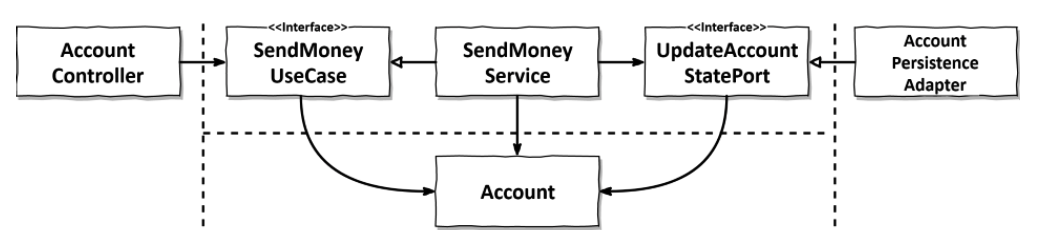
\includegraphics[height=0.1\textheight]{./part/Ejecucion/Seguimiento/CreateTaskUseCase/img/nomapping}
    \caption{No mapping strategy~\cite{TomHombergs2019GYHD}}\label{fig:nomapping}
\end{figure}

En la estrategia de \textit{No Mapping} ilustrada en la figura~\cref{fig:nomapping} se aprecia que tanto Aplicación como Infraestructura dependen de Dominio.
Esto evita todo código redundante, los \gls{DTO} (Data Transfer Object), pero resta flexibilidad.
Si por detalles técnicos de una Infraestructura concreta se requiere más o menos parámetros que los definidos en el Dominio, o se deben guardar en otro formato, este diseño se enfrenta a un problema.

\begin{figure}[H]
    \centering
    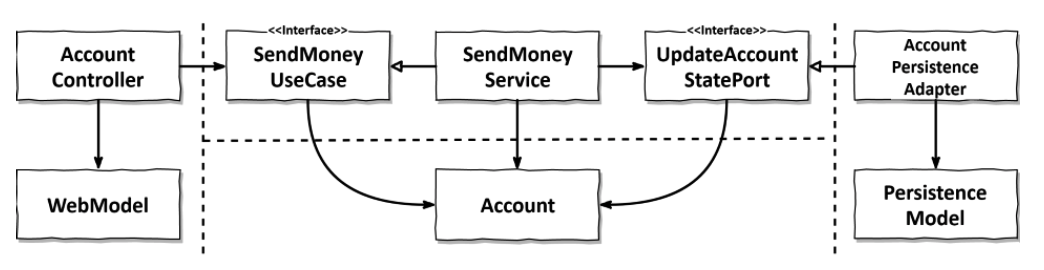
\includegraphics[height=0.1\textheight]{./part/Ejecucion/Seguimiento/CreateTaskUseCase/img/twowaymapping}
    \caption{Two way mapping strategy~\cite{TomHombergs2019GYHD}}\label{fig:twowaymapping}
\end{figure}

La estrategia de \textit{Two-Way Mapping Strategy}~\cref{fig:twowaymapping} evita este problema y crea un modelo DTO que sirva para transportar la información de una capa a otra necesaria para conformar la Entidad.
De esta forma puede evolucionar por separado.
El problema persiste entre la Aplicación, los casos de uso, y el Dominio.
Se hace necesario escribir más código para crear las entidades a través de los DTO y viceversa.

\begin{figure}[H]
    \centering
    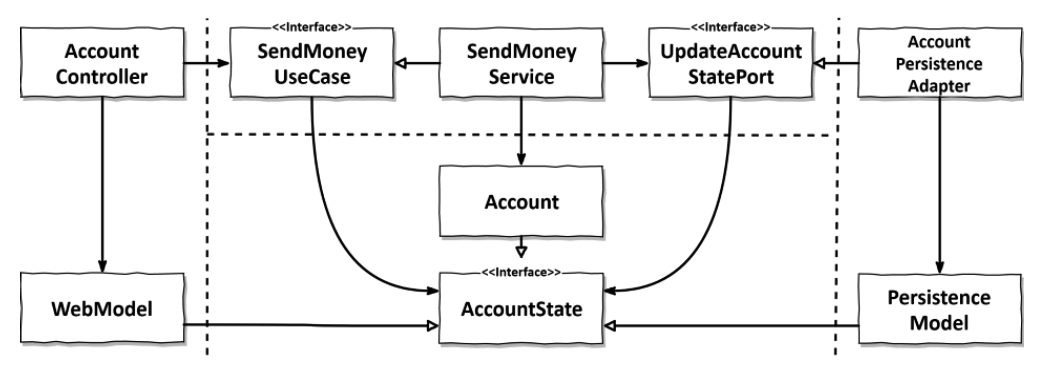
\includegraphics[height=0.1\textheight]{./part/Ejecucion/Seguimiento/CreateTaskUseCase/img/onWaymapping}
    \caption{One way mapping strategy~\cite{TomHombergs2019GYHD}}\label{fig:onWaymapping}
\end{figure}

En la estrategia de \textit{The One-Way Mapping Strategy}~\cref{fig:onWaymapping} se ilustra la creación de una interfaz para la Entidad y hace depender de nuevo todas las capas de dicha interfaz.
Se encuentran las capas más separadas y preparadas para el caso en el que se enfrente la necesidad de tener que crear distintas implementaciones aunque no se creen en un primer momento.

\begin{figure}[H]
    \centering
    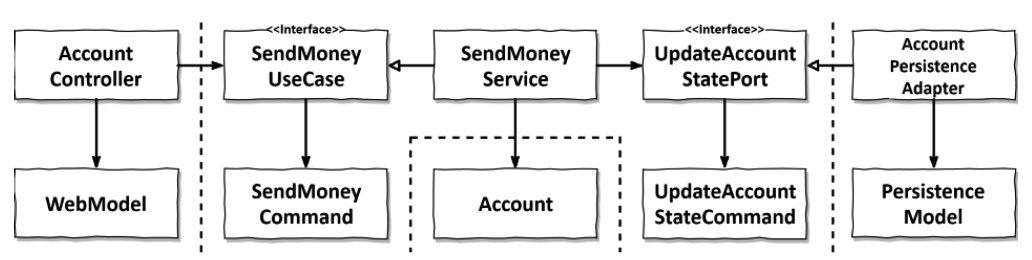
\includegraphics[height=0.1\textheight]{./part/Ejecucion/Seguimiento/CreateTaskUseCase/img/fullmapping}
    \caption{Full mapping strategy~\cite{TomHombergs2019GYHD}}\label{fig:fullmapping}
\end{figure}

En la figura de \textit{The Full Mapping Strategy}~\cref{fig:twowaymapping} se opta por crear DTOs entre todas las capas.
Es la solución más pura, pero el coste es evidente: la cantidad de código a realizar es considerable y tiene que estar justificada con una necesidad de aislar hasta este punto.

No hay una regla de oro para elegir una estrategia que valga para todos los casos.
Debe ser una decisión de equipo, seguir la decisión y re-evaluar con cada inconveniente que enfrente la decisión si se tiene que cambiar la estrategia.

Se puede ver el primer ejemplo en el un proyecto de ejecución que intentara resolver todas las decisiones y describir al detalle la solución a desarrollar no aportaría valor.
Tomar una decisión de este tipo y documentarla carece de utilidad en este punto del diseño;
no se dispone de información suficiente para ello.
Al enfrentar el desarrollo del código se podrá valorar qué estrategia encaja mejor.

\paragraph{\textit{Testing} o Testeo}
    Para el caso de uso de Create task siguiendo\ref{par:testing}

Primero tenemos que localizar los factores o variables independientes

\begin{itemize}
    \item Host
    \item Port
    \item CommunicationMode
    \item ExecutionMode
    \item Steps
\end{itemize}

luego las clases de equivalencia:

\begin{itemize}
    \item Host: valid/invalid
    \item Port: valid/invalid
    \item CommunicationMode: valid/invalid
    \item ExecutionMode: valid/invalid
    \item Steps: valid/invalid
\end{itemize}

Cabe reseñar que el trabajo de buscar las clases de equivalencia no es trivial. por ejemplo, en el caso de steps que es un array podría haberse pensado que se necesita probar con varios elementos en el array, validos e invalidos, pero no tiene sentido porque la lógica debe contemplar únicamente

o por ejemplo en el caso de Host o Port que tiene validaciones. podría pensarse que debería ponerse a prueba con varios casos que den invalido, al ser un string libre y que ponga a prueba dicha validación, pero estamos en el caso de uso, eso será responsabilidad del test unitario de Host y Port. para la lógica que nos atañe en este test lo único que importa es qué sucedera en el caso que sea válido o invalido.

En un ejemplo tan trivial puede llevar a subestimar el ejercicio de entender el alcance de la prueba y la correcta selección de las clases de equivalencia, pero es de suma importancia.

Bien pues con estas clases de equivalencia las posibilidades son \[ 2^5 = 32 \] casos con el método de pares se reduce a 6 y los pares posibles son 41

las combinaciones posibles son:

\begin{table}[H]
    \small
    \begin{tabular}{cccccc}
        \textbf{}   & \textbf{host} & \textbf{port} & \textbf{communicationMode} & \textbf{executionMode} & \textbf{sentences} \\
        \textbf{1}  & valid         & valid         & valid                      & valid                  & valid              \\
        \textbf{2}  & valid         & valid         & valid                      & valid                  & invalid            \\
        \textbf{3}  & valid         & valid         & valid                      & invalid                & valid              \\
        \textbf{4}  & valid         & valid         & valid                      & invalid                & invalid            \\
        \textbf{5}  & valid         & valid         & invalid                    & valid                  & valid              \\
        \textbf{6}  & valid         & valid         & invalid                    & valid                  & invalid            \\
        \textbf{7}  & valid         & valid         & invalid                    & invalid                & valid              \\
        \textbf{8}  & valid         & valid         & invalid                    & invalid                & invalid            \\
        \textbf{9}  & valid         & invalid       & valid                      & valid                  & valid              \\
        \textbf{10} & valid         & invalid       & valid                      & valid                  & invalid            \\
        \textbf{11} & valid         & invalid       & valid                      & invalid                & valid              \\
        \textbf{12} & valid         & invalid       & valid                      & invalid                & invalid            \\
        \textbf{13} & valid         & invalid       & invalid                    & valid                  & valid              \\
        \textbf{14} & valid         & invalid       & invalid                    & valid                  & invalid            \\
        \textbf{15} & valid         & invalid       & invalid                    & invalid                & valid              \\
        \textbf{16} & valid         & invalid       & invalid                    & invalid                & invalid            \\
        \textbf{17} & invalid       & valid         & valid                      & valid                  & valid              \\
        \textbf{18} & invalid       & valid         & valid                      & valid                  & invalid            \\
        \textbf{19} & invalid       & valid         & valid                      & invalid                & valid              \\
        \textbf{20} & invalid       & valid         & valid                      & invalid                & invalid            \\
        \textbf{21} & invalid       & valid         & invalid                    & valid                  & valid              \\
        \textbf{22} & invalid       & valid         & invalid                    & valid                  & invalid            \\
        \textbf{23} & invalid       & valid         & invalid                    & invalid                & valid              \\
        \textbf{24} & invalid       & valid         & invalid                    & invalid                & invalid            \\
        \textbf{25} & invalid       & invalid       & valid                      & valid                  & valid              \\
        \textbf{26} & invalid       & invalid       & valid                      & valid                  & invalid            \\
        \textbf{27} & invalid       & invalid       & valid                      & invalid                & valid              \\
        \textbf{28} & invalid       & invalid       & valid                      & invalid                & invalid            \\
        \textbf{29} & invalid       & invalid       & invalid                    & valid                  & valid              \\
        \textbf{30} & invalid       & invalid       & invalid                    & valid                  & invalid            \\
        \textbf{31} & invalid       & invalid       & invalid                    & invalid                & valid              \\
        \textbf{32} & invalid       & invalid       & invalid                    & invalid                & invalid
    \end{tabular}
    \caption{tab:table2}\label{tab:table2}
\end{table}

y los pares son

\begin{table}[H]
    \small
    \begin{tabular}{llll}
        \textbf{var1}          & \textbf{var2}     & \textbf{value1} & \textbf{value2} \\
        \textbf{host}          & port              & valid           & valid           \\
        \textbf{host}          & port              & valid           & notValid        \\
        \textbf{host}          & port              & notValid        & valid           \\
        \textbf{host}          & port              & notValid        & notValid        \\
        \textbf{host}          & executionMode     & valid           & valid           \\
        \textbf{host}          & executionMode     & valid           & notValid        \\
        \textbf{host}          & executionMode     & notValid        & valid           \\
        \textbf{host}          & executionMode     & notValid        & notValid        \\
        \textbf{host}          & communicationMode & valid           & valid           \\
        \textbf{host}          & communicationMode & valid           & notValid        \\
        \textbf{host}          & communicationMode & notValid        & valid           \\
        \textbf{host}          & communicationMode & notValid        & notValid        \\
        \textbf{host}          & steps             & valid           & valid           \\
        \textbf{host}          & steps             & valid           & notValid        \\
        \textbf{host}          & steps             & notValid        & valid           \\
        \textbf{host}          & steps             & notValid        & notValid        \\
        \textbf{port}          & executionMode     & valid           & valid           \\
        \textbf{port}          & executionMode     & valid           & notValid        \\
        \textbf{port}          & executionMode     & notValid        & valid           \\
        \textbf{port}          & executionMode     & notValid        & notValid        \\
        \textbf{port}          & communicationMode & valid           & valid           \\
        \textbf{port}          & communicationMode & valid           & notValid        \\
        \textbf{port}          & communicationMode & notValid        & valid           \\
        \textbf{port}          & communicationMode & notValid        & notValid        \\
        \textbf{port}          & steps             & valid           & valid           \\
        \textbf{port}          & steps             & valid           & notValid        \\
        \textbf{port}          & steps             & notValid        & valid           \\
        \textbf{port}          & steps             & notValid        & notValid        \\
        \textbf{executionMode} & communicationMode & valid           & valid           \\
        \textbf{executionMode} & communicationMode & valid           & notValid        \\
        \textbf{executionMode} & communicationMode & notValid        & valid           \\
        \textbf{executionMode} & communicationMode & notValid        & notValid        \\
        executionMode          & steps             & valid           & valid           \\
        executionMode          & steps             & valid           & notValid        \\
        executionMode          & steps             & notValid        & valid           \\
        executionMode          & steps             & notValid        & notValid        \\
        communicationMode      & steps             & valid           & valid           \\
        communicationMode      & steps             & valid           & notValid        \\
        communicationMode      & steps             & notValid        & valid           \\
        communicationMode      & steps             & notValid        & notValid
    \end{tabular}
    \caption{tab:table3}\label{tab:table3}
\end{table}

El tests quedaría entonces como sale en la figura \ref{tab:createTaskPairWiseTest}

\begin{table}[H]
    \small
    \begin{tabular}{rllllll}
        case & host     & port     & ExeMode  & ComMode  & steps    & Expected Result        \\
        1    & valid    & valid    & valid    & valid    & valid    & OK                     \\
        2    & valid    & notValid & notValid & notValid & notValid & PortInvalidError       \\
        3    & notValid & valid    & notValid & valid    & notValid & HostInvalidError       \\
        4    & notValid & notValid & valid    & notValid & valid    & HostInvalidError       \\
        5    & ~valid   & valid    & valid    & notValid & notValid & CommunicationModeError \\
        6    & ~valid   & notValid & notValid & valid    & valid    & PortError
    \end{tabular}
    \caption{tab:createTaskPairWiseTest}\label{tab:createTaskPairWiseTest}
\end{table}

En la instaciación de una nueva Task tenemos los

Primero tenemos que localizar los factores o variables independientes

\begin{itemize}
    \item Number of steps
    \item execution Mode
    \item Communication Mode
\end{itemize}

luego las clases de equivalencia:

\begin{itemize}
    \item NSteps: 0,1,>2
    \item ExMod: Automatic, Manual
    \item ComMode: Server Stream,Client Stream, Bidirectional y Unary
\end{itemize}

tenemos entonces \[ 3*2*4 = 24 \] posibilidades pares obtenemos 27 al final queda reducidos a 13 casos. Vemos que la eficiencia en reducción de casos disminuye cuanto menos combinaciones hay. El diseño de los tests queda tal y como se ve en la tabla \ref{tab:taskTestPairwiseCases}

\begin{table}[H]
    \small
    \begin{tabular}{ccccl}
        \textbf{}   & \textbf{NSteps} & \textbf{ExeMod} & \textbf{ComMode} & \multicolumn{1}{c}{\textbf{Expected Result}}  \\
        \textbf{1}  & 0               & automatic       & serverStream     & NewTaskMustHaveAtLeastOneStepError            \\
        \textbf{2}  & 1               & automatic       & clientStream     & OK                                            \\
        \textbf{3}  & 1               & manual          & bidirectional    & OK                                            \\
        \textbf{4}  & 1               & automatic       & unary            & OK                                            \\
        \textbf{5}  & 1               & manual          & serverStream     & OK                                            \\
        \textbf{6}  & \textgreater{}2 & manual          & unary            & CommunicationModeCanOnlyHaveOneStepError      \\
        \textbf{7}  & \textgreater{}2 & automatic       & serverStream     & CommunicationModeCanOnlyHaveOneStepError      \\
        \textbf{8}  & \textgreater{}2 & manual          & clientStream     & OK                                            \\
        \textbf{9}  & \textgreater{}2 & automatic       & bidirectional    & ManualBidirectionalTaskOnlyCanHave2StepsError \\
        \textbf{10} & 0               & automatic       & clientStream     & TaskMustHaveAtLeastOneStepError               \\
        \textbf{11} & 0               & manual          & bidirectional    & TaskMustHaveAtLeastOneStepError               \\
        \textbf{12} & 0               & automatic       & unary            & TaskMustHaveAtLeastOneStepError               \\
        \textbf{13} & 0               & manual          & serverStream     & TaskMustHaveAtLeastOneStepError
    \end{tabular}
    \caption{tab:taskTestPairwiseCases}\label{tab:taskTestPairwiseCases}
\end{table}

Ahora vamos a ver cómo la arquitectura protege la calidad del sistema de las implementaciones en proceso de investigación. Sabemos que el looper tiene los siguientes factores:

\begin{figure}[H]
    \centering
    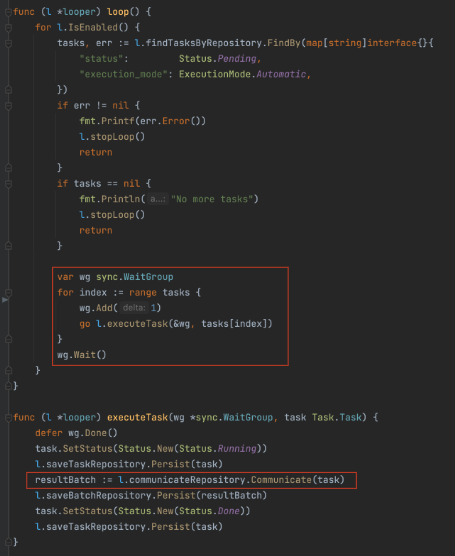
\includegraphics[height=0.3\textheight]{./part/Ejecucion/Seguimiento/Testing/img/Looper}
    \caption{testing looper.go detail}\label{fig:testingLooper}
\end{figure}

el punto clave de la figura \ref{fig:testingLooper} señalado en el recuadro rojo es el adaptador de comunicación GRPC es un adaptador experimental que debido a la inexperiencia en su uso está desarrollado de forma ineficiente. Hemos extraido toda la lógica posible a este servicio que es la parte core:

El adaptador puede tener múltiples errores inesperados, no conseguir comunicar con el servicio cliente, timeouts, malas implementaciones de la librería, pero se ha protegido al dominio de todo esto mediante una interfaz que garantiza que ante cualquier error se devuelve siempre un resultado. Lo único que quedaría por implementar y testear sería que el proceso no consiguiera terminar y se quedara la gorutine en un proceso infinito. para ello en el proceso de descubrimiento del lenguaje sabemos que hay un punto débil en el dominio. No hemos hehco uso de una herramienta de Golang que se conoce como context. que permite gestionar los timeouts de las gorutines evitando que que queden procesos hijos sin control.

Tengamos en cuenta que hemos extraido de toda la comunicación con el cliente una interfaz útil y única para comunicarnos, una lógica de negocio que entender en pocas lineas de código y explicar su funcionamiento, controlarlo y testearlo y aún así encontramos puntos débiles que mejorar en ese diseño. Si a esto le hubieramos sumado las lineas de codigo que hay detrás de la interfaz de comunicacion sería ingestionable. para cuantificar esto vamos a hacer una aproximación al diseño del test necesario para cubrir el adaptador de comunicacion

El código completo se encuentra en el repositorio github. Simplificando para esta explicación el pseudocódigo sería el siguiente

\begin{verbatim}
connection, err := grpc.Dial()
    serverStream:
        client.CallServerStream(request)
        responseStream.Recv()
    Bidirectional:
        client.CallBidirectional()
        async stream.Recv()
        async stream.Send()
        stream.CloseSend()
    ClientStream:
        client.CallClientStream()
        stream.Send
        stream.CloseAndRecv()
    Unary
        client.CallUnary()
connection.Close()
\end{verbatim}

vemos que hay mucha lógica junta, múltiples responsabilidades y por lo tanto no es un buen diseño. Como se demuestra mejor es intentando diseñar los tests. Para empezar extraer del código estas clases de equivalencia y factores no ha sido sencillo ya que hay multiples gestiones de errores dispersos por el código y es un código extenso 178 lineas. Esto ocurre en multitud de ocasiones, ya sea debido al tiempo, desconocimiento o mala praxis nos encontramos con códigos de esta magnitud. La arquitectura y todo este proceso lo que hace es protegernos de estas secciones sucias.

factores y posibles respuestas:

\begin{itemize}
    \item grpc.Dial(): err, connection
    \item client.CallServerStream(request): err,stream
    \item responseStream.Recv(): EOF,err,nil
    \item client.CallBidirectional(): error,stream
    \item stream.Recv(): EOF,err, result
    \item stream.Send(): EOF, nil,err
    \item stream.CloseSend() err,nil
    \item client.CallClientStream(): err, stream
    \item stream.Send: err, nil
    \item stream.CloseAndRecv(): err, nil
    \item client.CallUnary(): err,nil
    \item connection.Close(): err, nil
\end{itemize}

Si no entendieramos bien el concepto de clase de equivalencia podría llevarnos a un mal diseño de los tests o a hacerlo más complejo. Aunque hay factores que tiene tres respuestas posibles EOF y nil tienen que ir de la mano, significa que no ha habido error, primero obtienes un nil en el error y luego obtienes un error tipo EOF que significa que todo ha terminado correctamente. y luego tenemos cuando obtenmos un error distinto de EOF, si esto ocurre nos importa cuaántas veces haya ocurrido el caso sin error, será error igualmente. Con lo cual las clases de equivalencia serían

\begin{itemize}
    \item grpc.Dial(): err, connection
    \item client.CallServerStream(): err,stream
    \item responseStream.Recv(): nil\&EOF,err
    \item client.CallBidirectional(): error,stream
    \item stream.Recv(): nil\&EOF,err
    \item stream.Send(): nil\&EOF,err
    \item stream.CloseSend() err,nil
    \item client.CallClientStream(): err, stream
    \item stream.Send: err, nil
    \item stream.CloseAndRecv(): err, nil
    \item client.CallUnary(): err,nil
    \item connection.Close(): err, nil
\end{itemize}

para este caso tendríamos \[ 2^{12} = 4096 \] combinaciones posibles que pairwise reduce a 59 tests. aquí se ve la potencia del método. Volviendo posible un testing con ciertas garantías incluso en un código como el que nos ocupa.


\paragraph{Docker}

Docker es el sistema de gestión de contenedores más utilizado en la industria a día de hoy.
Según la misma página oficial de Docker un contenedor se define como: Una unidad estándar de software que empaqueta el código y todas sus dependencias de tal modo que la aplicación pueda ejecutarse de forma rápida y fiable de un entorno de ejecución a otro.
La imagen de un contenedor es un paquete de software ligero, independiente y ejecutable que incluye todo lo que necesita para ser ejecutado: el código, el sistema, las herramientas, librerías y configuración~\cite{docker}.

El sistema se basa en la definición de imágenes que no son más que las instrucciones para la construcción de esos contenedores mediante el sistema de Docker Engine.
Difieren de las máquinas virtuales tal y como se muestra en la comparativa~\cref{fig:Docker vs VM}.

Esto permite correr multiples aplicaciones con multiples requerimientos en cualquier máquina sin tener que instalar dichas dependencias de forma local, evitando incompatibilidades e interacciones no deseadas.
Permite ofrecer un producto consistentes a los clientes de forma que el software y todo aquello que necesita para ejecutarse se entregan de forma conjunta, evitando problemas de instalación.

\begin{figure}[H]
    \centering
    \includegraphics[height=0.3\textheight]{./part/Proyecto_ejecutivo/memoria_descriptiva/prestaciones/docker/img/dockerVsVM}
    \caption{Comparación: Docker vs Máquinas virtuales.\cite{docker}}\label{fig:Docker vs VM}
\end{figure}

En la~\cref{fig:Docker vs VM} se muestra una comparación entre las capas que virtualiza cada sistema.
Cada contenedor de Docker es una abstracción en la capa de aplicación que empaqueta el código y las dependencias juntas.
Múltiples contenedores pueden ejecutarse en la misma máquina y compartir el \textit{Kernel} del sistema operativo cada uno ejecutándose en un entorno completamente aislado.
Los contenedores utilizan menos espacio que las máquinas virtuales, pueden manejar más aplicaciones y requieren menos virtualización y requerimientos del sistema operativo que otros sistemas.

Las máquinas virtuales son una abstracción completa del sistema físico que emulan, el hardware.
Sirven para transformar una máquina en, virtualmente, múltiples máquinas.
Cada máquina virtual incluye una copia completa de un sistema operativo, la aplicación, los ejecutables y librerías;
llegando a ocupar Gigas y sus arranques son lentos.

Los principales beneficios del sistema Docker son que:
\begin{itemize}
    \item Permite trabajar en el desarrollo de distintos proyectos con distintos requerimientos en una misma máquina sin la complejidad de mantener las dependencias de cada proyecto.
    O trasladarse a otra máquina y seguir trabajando de forma rápida al no tener que ponerse a instalar dichas dependencias de nuevo.
    \item Permite trabajar en equipo ya que cada cambio en las dependencias queda expresado en los cambios que se realizan de las imágenes de los contenedores que están disponibles para todo el equipo.
    \item Permite configurar el sistema para desarrollar o para producción de forma consistente con sus distintas diferencias en las dependencias necesarias, evitando problemas en el cambio de entorno de desarrollo y producción.
\end{itemize}